\documentclass{article}

\usepackage{amsmath}
\usepackage[T1]{fontenc}
\usepackage[margin=2.5cm]{geometry}
\usepackage{comment}
\usepackage{graphicx}
\usepackage{float}


\begin{document}
\section{Introduction}
\subsection{The problem of aerodynamic drag}
Dlaczego badamy oraz wzór na opór aerodynamiczny. Że bazujemy na modern exterior balistics i jakieś inne z literatury bo to łądnie brzmi.

\begin{comment}
\subsection{Methodology of the present work}
For simulations we choose two programs to compare the results. The first one is 
Solidworks Flow Simulation, in which we also prepared models for simulations. 
The second one is Ansys Fluent.\\\\
First we prepared the models in Solidworks and from there we exported them to 
.step (214) file format to import them to Ansys. In Ansys we used Fluent with
Meshing to prepare the mesh and then we run the simulations. Solidworks Flow Simulation
was also used to prepare the mesh and run the simulations, which we later compared with
Ansys Fluent results.\\\\
All models were tested using Parametric studies/sets for 9 different velocities 
from 0.1 to 1.0. The resulting graphs of drag coefficient vs mach number were 
compared and analyzed.
\end{comment}

\subsection{Methodology of the present work}
For simulations, two programs were chosen to compare the results. The first program, 
Solidworks Flow Simulation, was used for both CFDs and model preparation. The second 
program utilized was Ansys Fluent.\\\\
Initially, the models were prepared in Solidworks and subsequently exported to 
.step (214) file format for importation into Ansys. Within Ansys, Fluent with 
Meshing was used to prepare the mesh, followed by the execution of simulations. 
Solidworks Flow Simulation was also employed for mesh preparation and simulation execution, 
enabling subsequent comparison with results obtained from Ansys Fluent.\\\\
Parametric studies/sets were conducted for all models, encompassing nine different velocities
ranging from 0.1 to 1.0. Subsequently, resulting graphs depicting the drag coefficient 
versus Mach number were analyzed and compared.



\subsection{Tested models}
R6-Endcone, R6-No-Endcone, PrawieR5\\\\
For each set of simulations, computational domain mesh setting and graph of velocity and 
pressure for 0.6 mach will be shown.\\\\

\section{Initial study}
ChatGPT

The work was initiated with the remodeled R5 model, which had been prepared in Solidworks 
and featured an endcone, a modification in comparison to the original R5 model. Subsequent 
testing of the model was conducted using Solidworks Flow Simulation. However, this model 
was solely utilized for comparing the results of the older model with the new one. The 
results can be observed here

\begin{figure}[H]
    \centering
    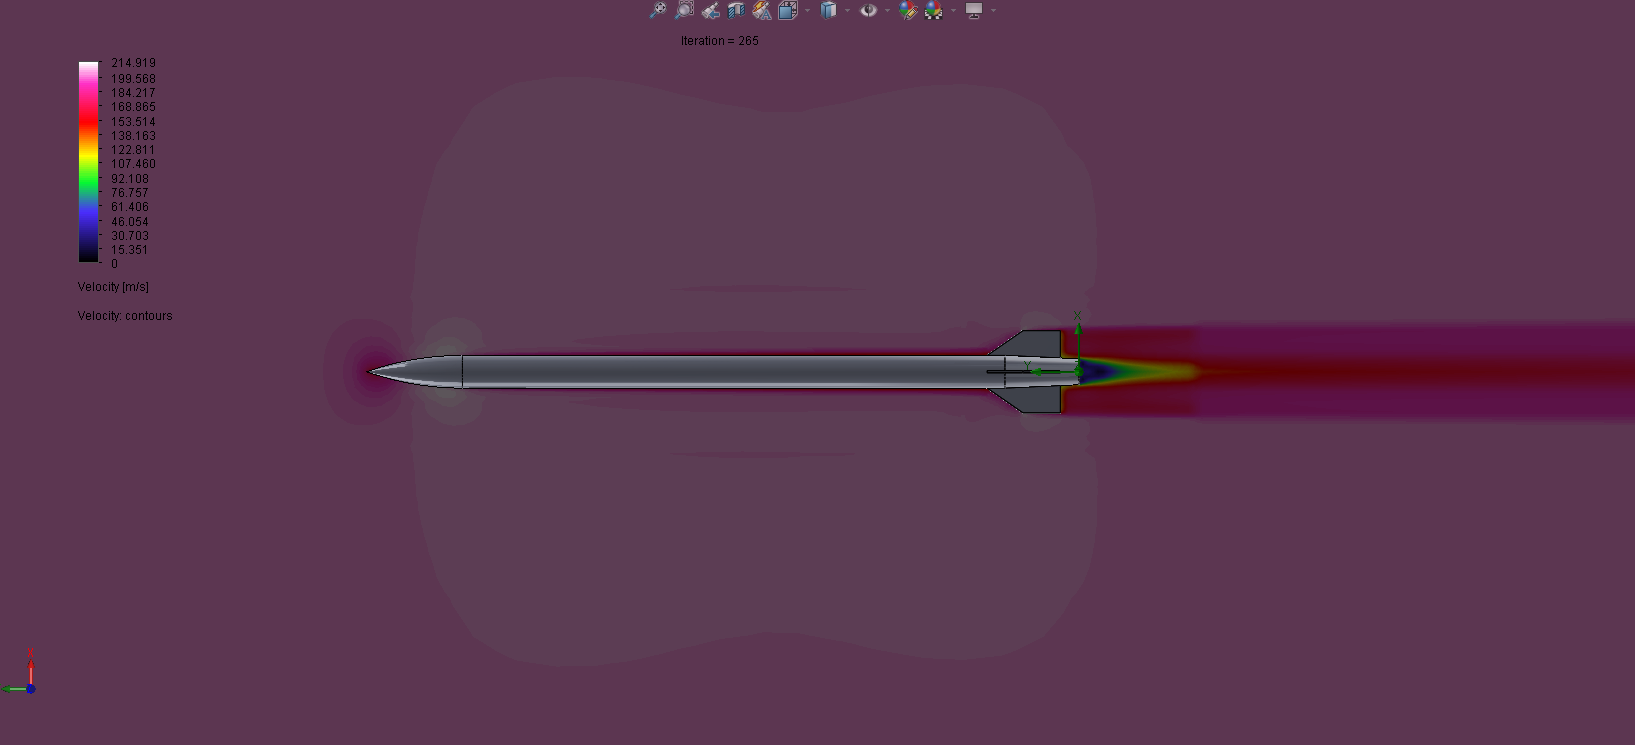
\includegraphics[width=\textwidth]{../data/PrawieR5-Solid/PrawieR5-TR-Velocity-Mach06.png}
    \caption{Velocity graph for PrawieR5 model at Mach 0.6}
\end{figure}

\begin{figure}[H]
    \centering
    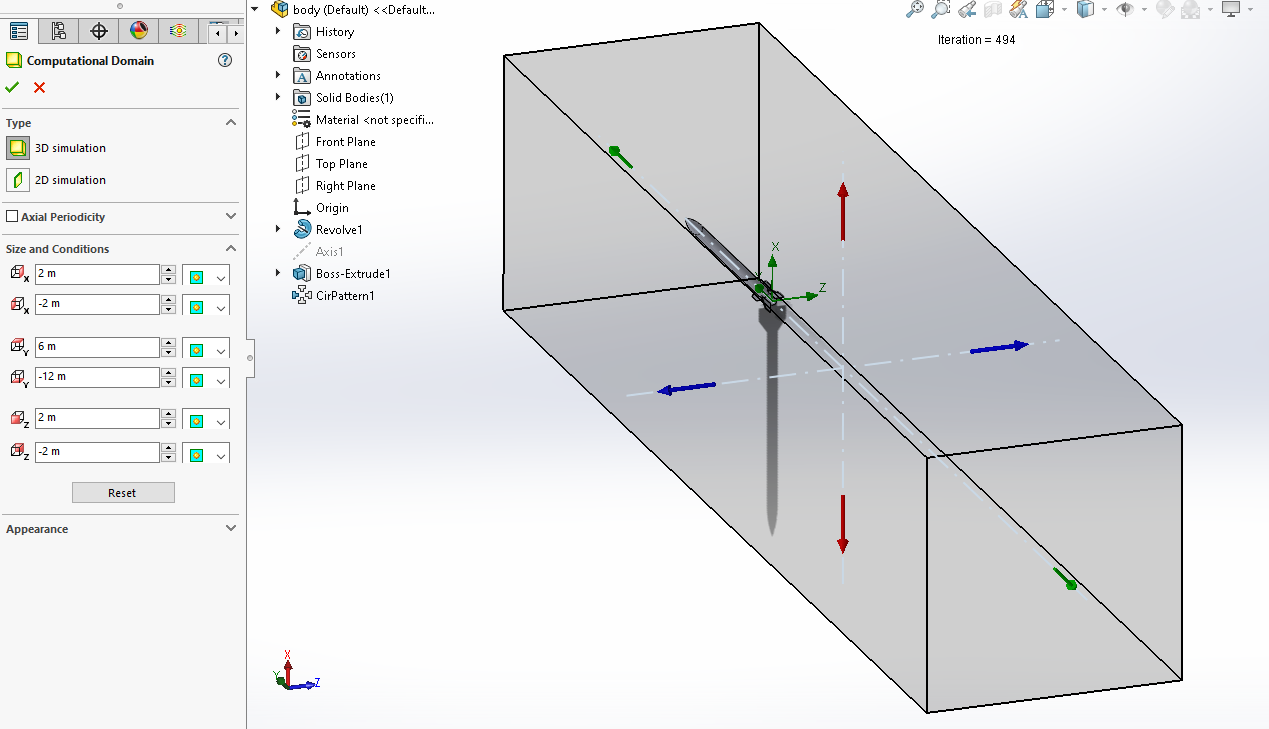
\includegraphics[width=\textwidth]{../data/PrawieR5-Solid/ComputationalDomain.png}
    \caption{CD graph for PrawieR5 model at Mach 0.6}
\end{figure}


\section{Preliminary research of endcone effect in Solidworks}
\subsection{R6 Endcone}
\begin{figure}[H]
    \centering
    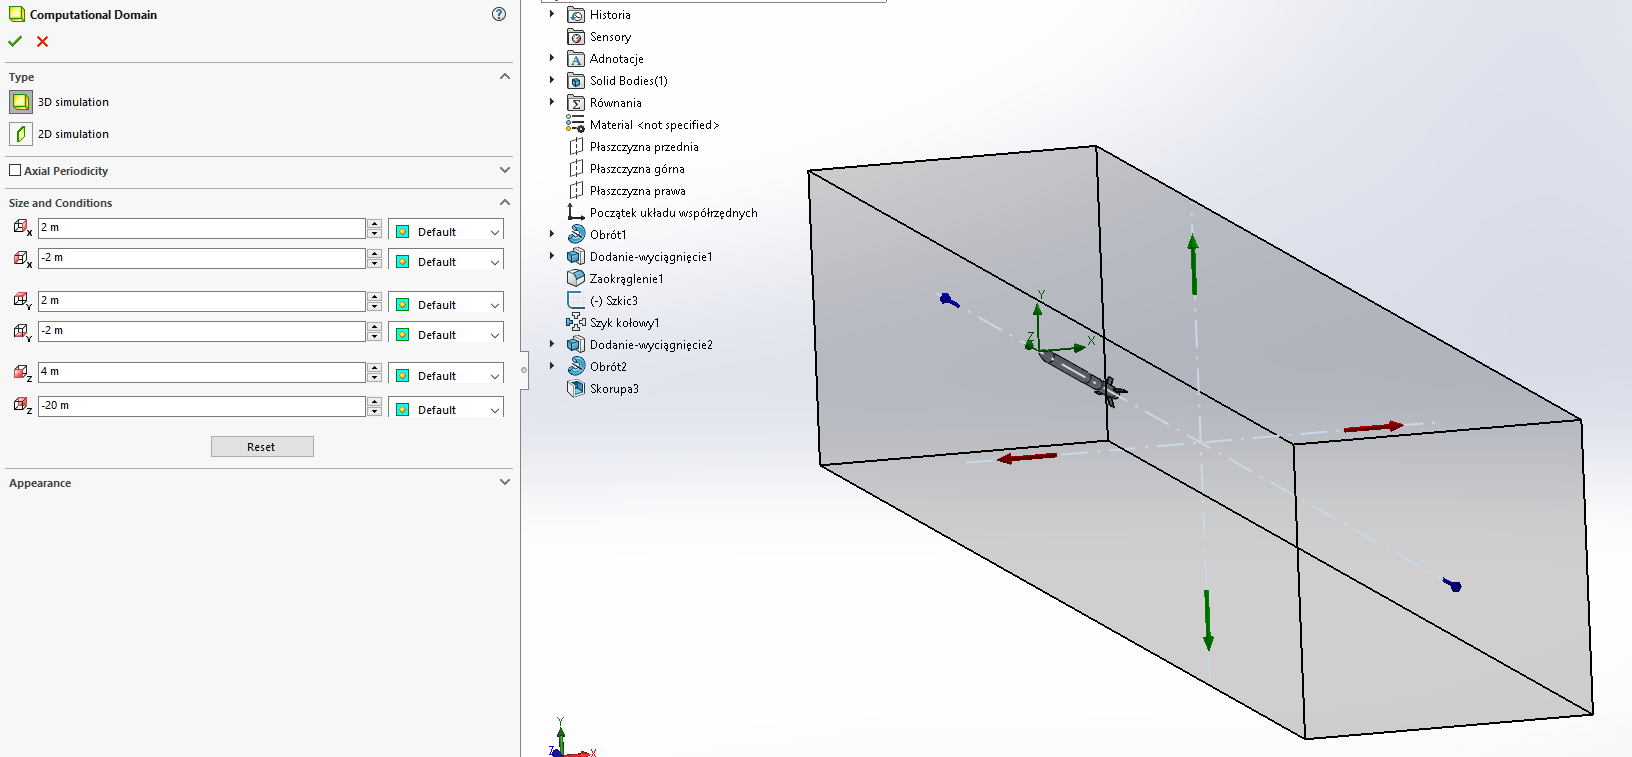
\includegraphics[width=\textwidth]{../data/R6-Endcone-Solid/domain.png}
    \caption{Computational domain for R6-Endcone model}
\end{figure}
\begin{figure}[H]
    \centering
    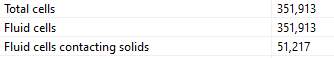
\includegraphics[width=0.6\textwidth]{../data/R6-Endcone-Solid/cells.png}
    \caption{Cell number for R6-Endcone model}
\end{figure}

\begin{figure}[H]
    \centering
    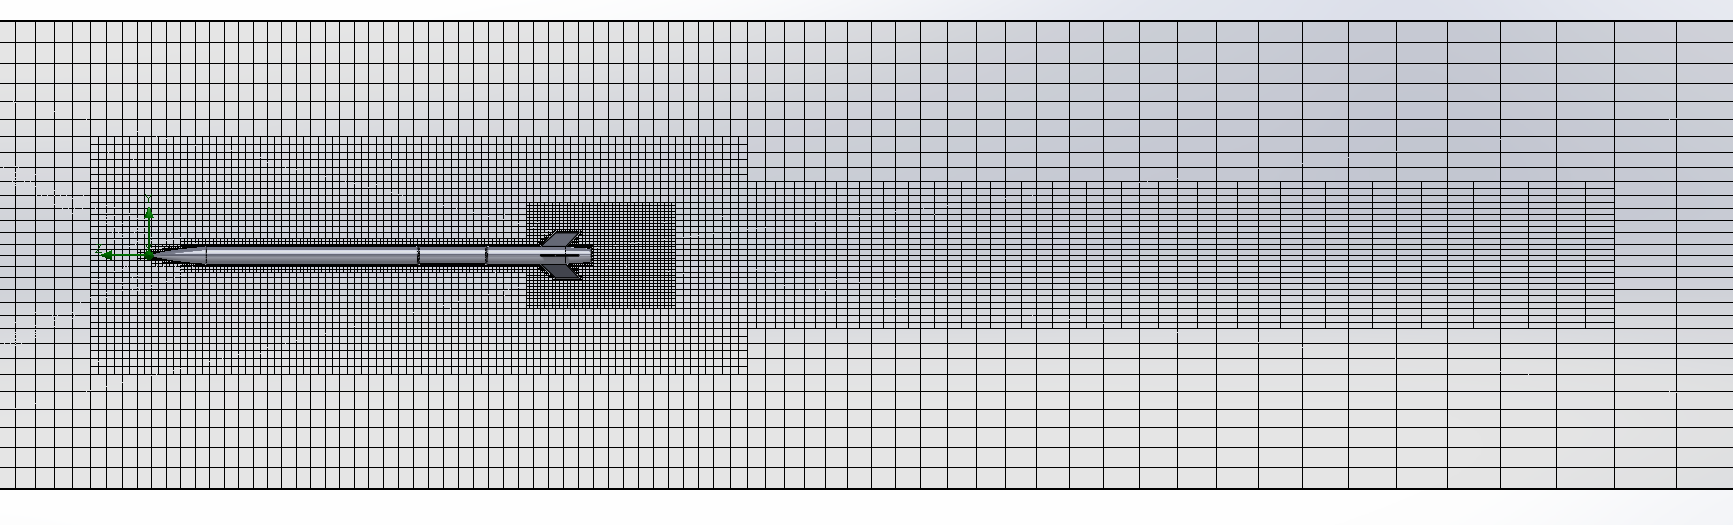
\includegraphics[width=\textwidth]{../data/R6-Endcone-Solid/mesh.png}
    \caption{Mesh for R6-Endcone model}
\end{figure}
\begin{figure}[H]
    \centering
    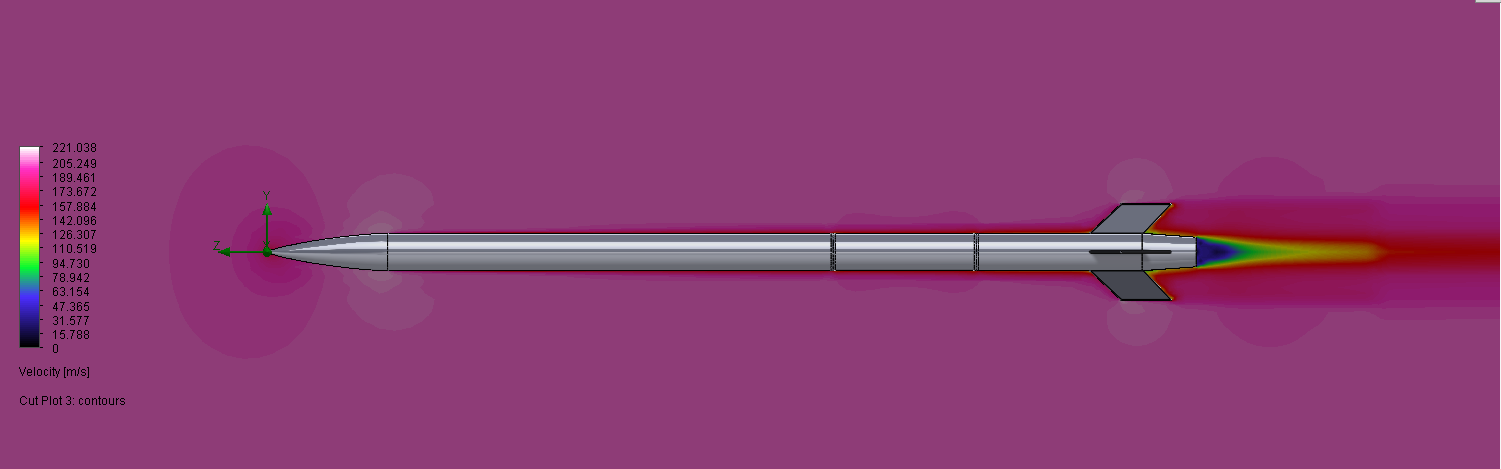
\includegraphics[width=\textwidth]{../data/R6-Endcone-Solid/speed.png}
    \caption{Velocity graph at 0.6 Mach for R6-Endcone model}
\end{figure}

\begin{figure}[H]
    \centering
    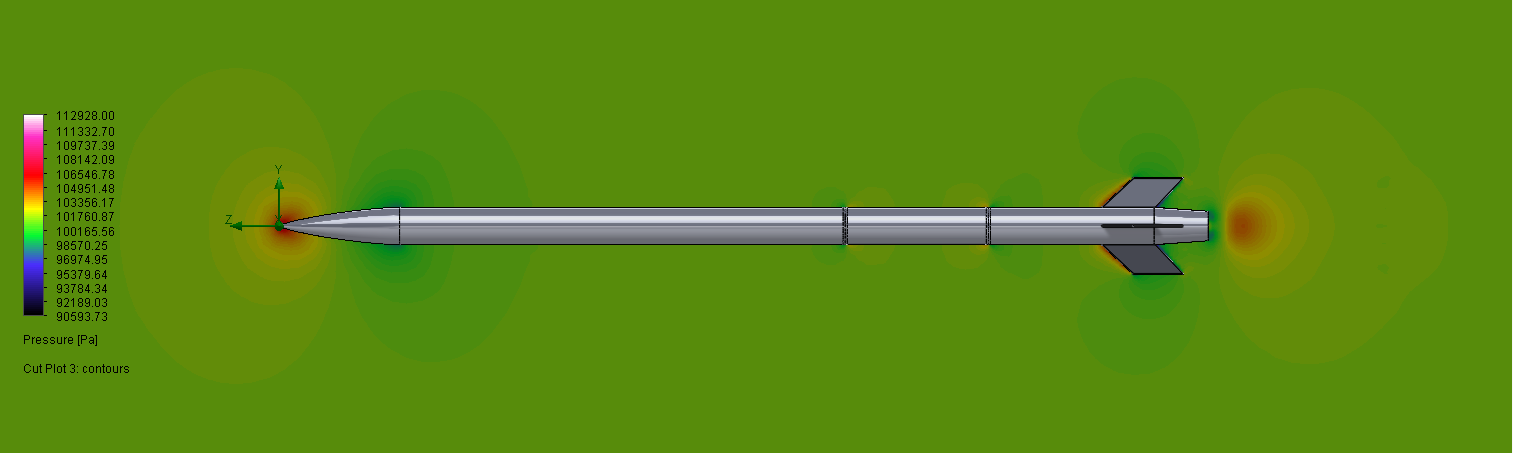
\includegraphics[width=\textwidth]{../data/R6-Endcone-Solid/pressure.png}
    \caption{Pressure graph at 0.6 Mach for R6-Endcone model}
\end{figure}

\subsection{R6 No Endcone}

\begin{figure}[H]
    \centering
    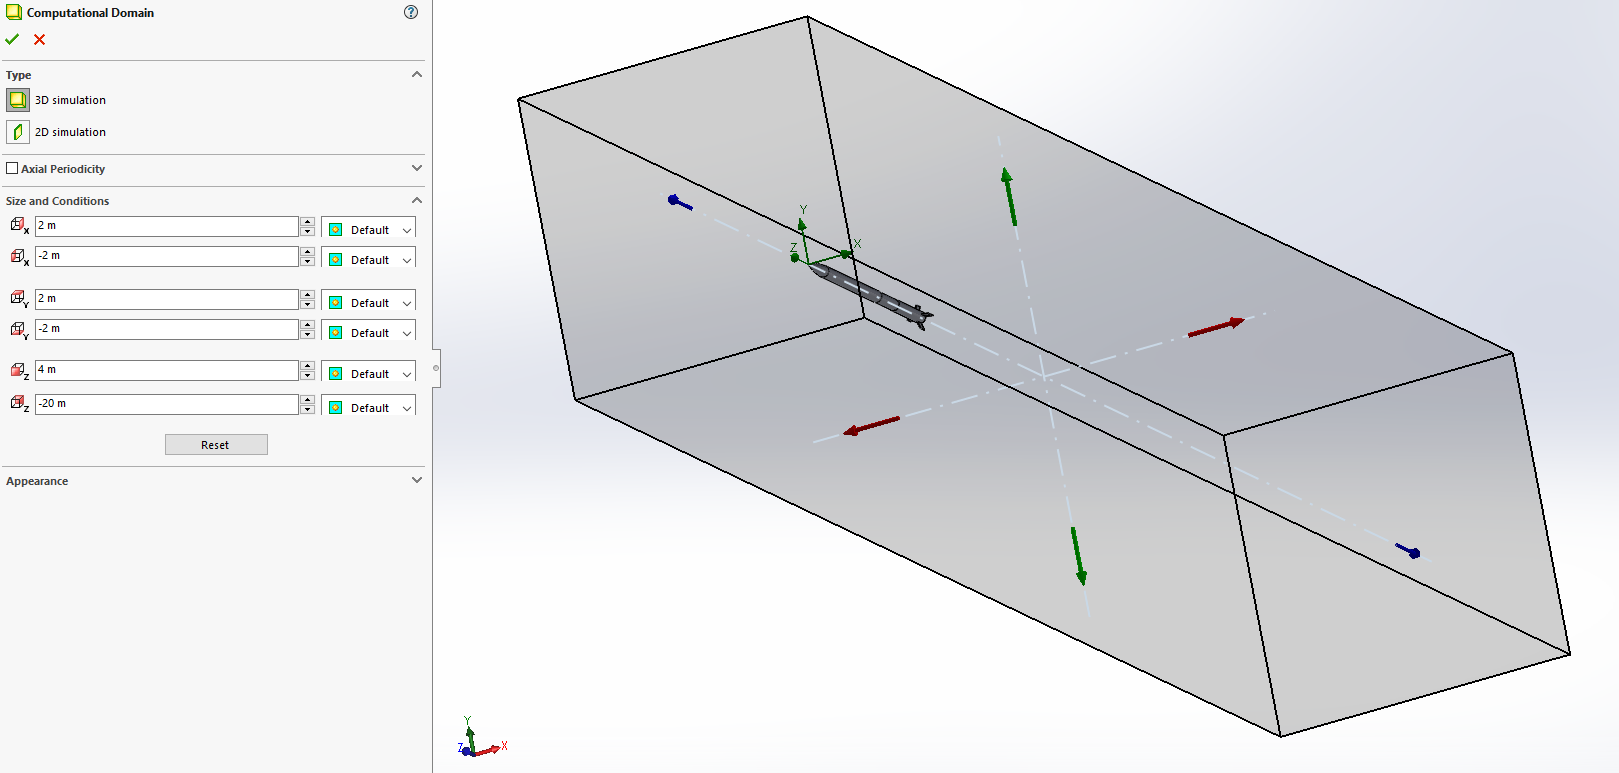
\includegraphics[width=\textwidth]{../data/R6-NoEndcone-Solid/domain.png}
    \caption{Computational domain for R6-NoEndcone model}
\end{figure}
\begin{figure}[H]
    \centering
    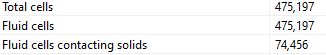
\includegraphics[width=0.6\textwidth]{../data/R6-NoEndcone-Solid/cells.png}
    \caption{Cell number for R6-NoEndcone model}
\end{figure}

\begin{figure}[H]
    \centering
    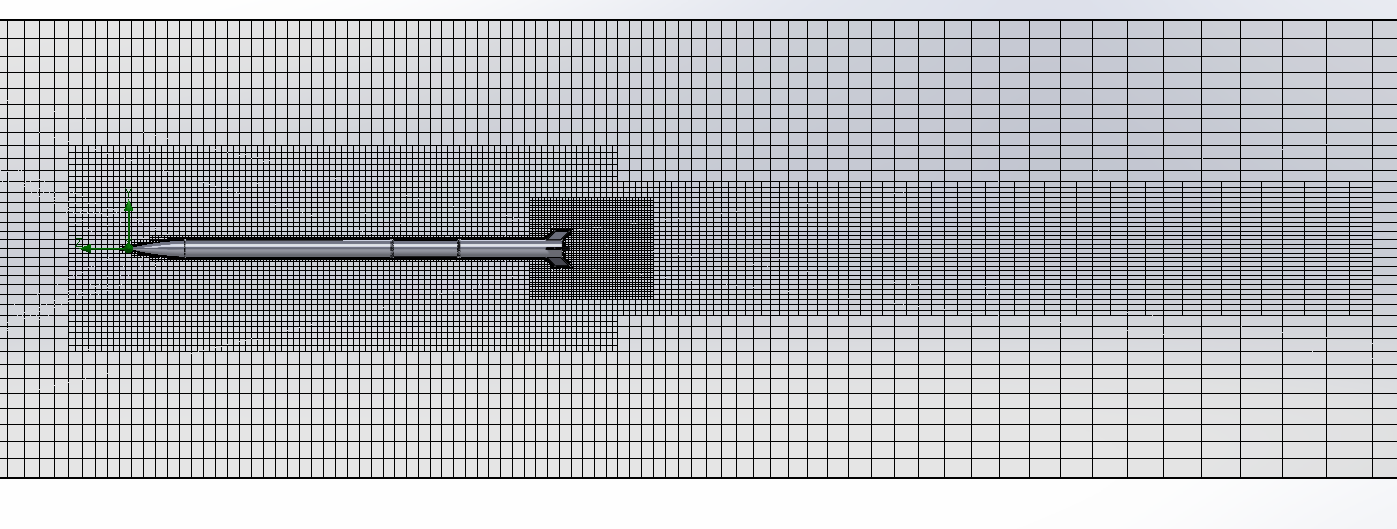
\includegraphics[width=\textwidth]{../data/R6-NoEndcone-Solid/mesh.png}
    \caption{Mesh for R6-NoEndcone model}
\end{figure}
\begin{figure}[H]
    \centering
    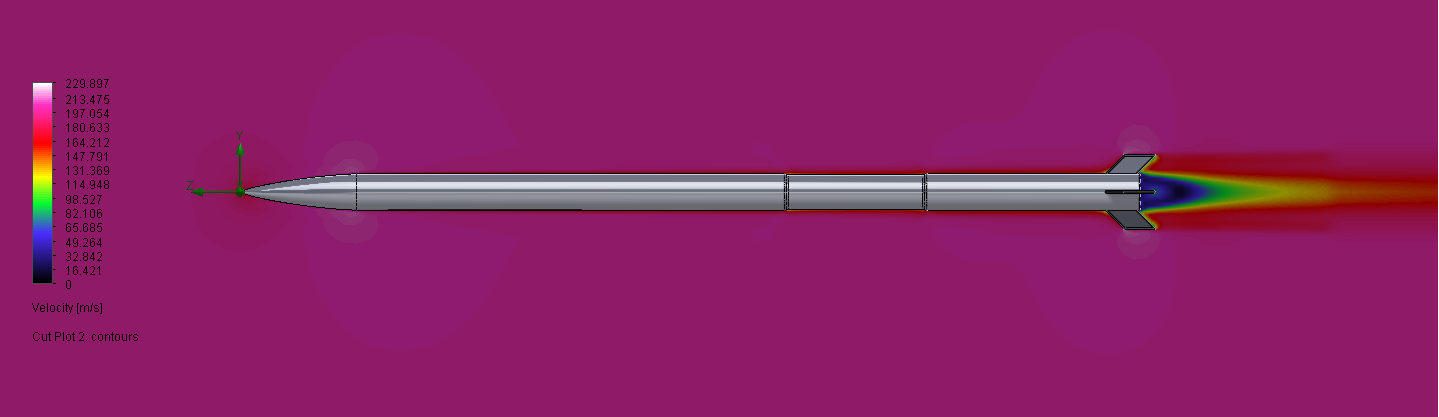
\includegraphics[width=\textwidth]{../data/R6-NoEndcone-Solid/speed.png}
    \caption{Velocity graph at 0.6 Mach for R6-NoEndcone model}
\end{figure}

\begin{figure}[H]
    \centering
    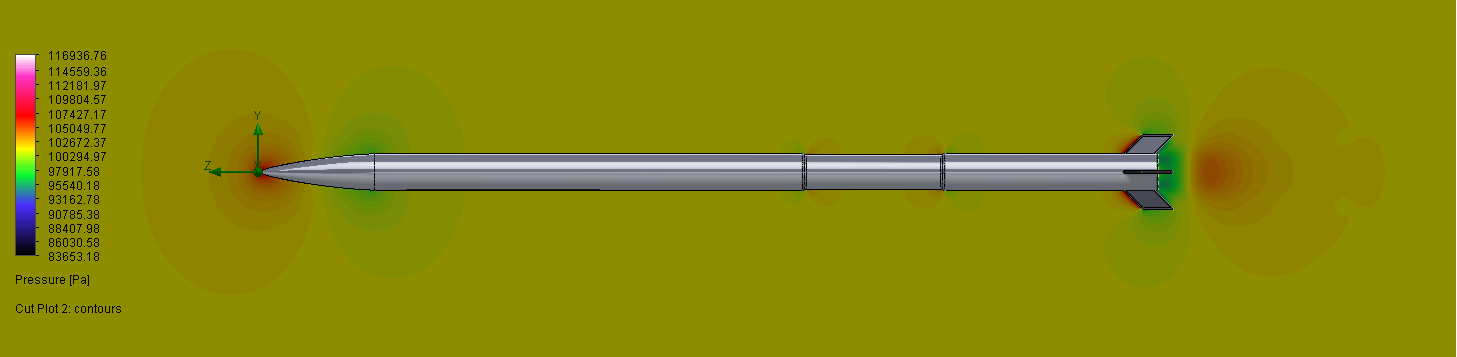
\includegraphics[width=\textwidth]{../data/R6-NoEndcone-Solid/konospeedoatode.png}
    \caption{Pressure graph at 0.6 Mach for R6-NoEndcone model}
\end{figure}

\subsection{Results of the preliminary research}


\section{Results and discussion}
\begin{itemize}
    \item Wykresy CD solida
    \item Wykres CD fluenta
    \item porównanie CD dla wyników solida i ansysa jakąś tam statystyką z użyciem pythona(ja to zrobie)
    \item Podsumowanie że wyszedł lepszy dla endcone(co się zgadza z literaturą i przewidywaniami) 
    oraz jakieś tam gadu gadu o Solidzie że gorszy. 
\end{itemize}

\end{document}